\chapter{Practical work}\label{cha:work} % chktex 24


\section{Material plots?}
\begin{figure}[H]
    \centering
    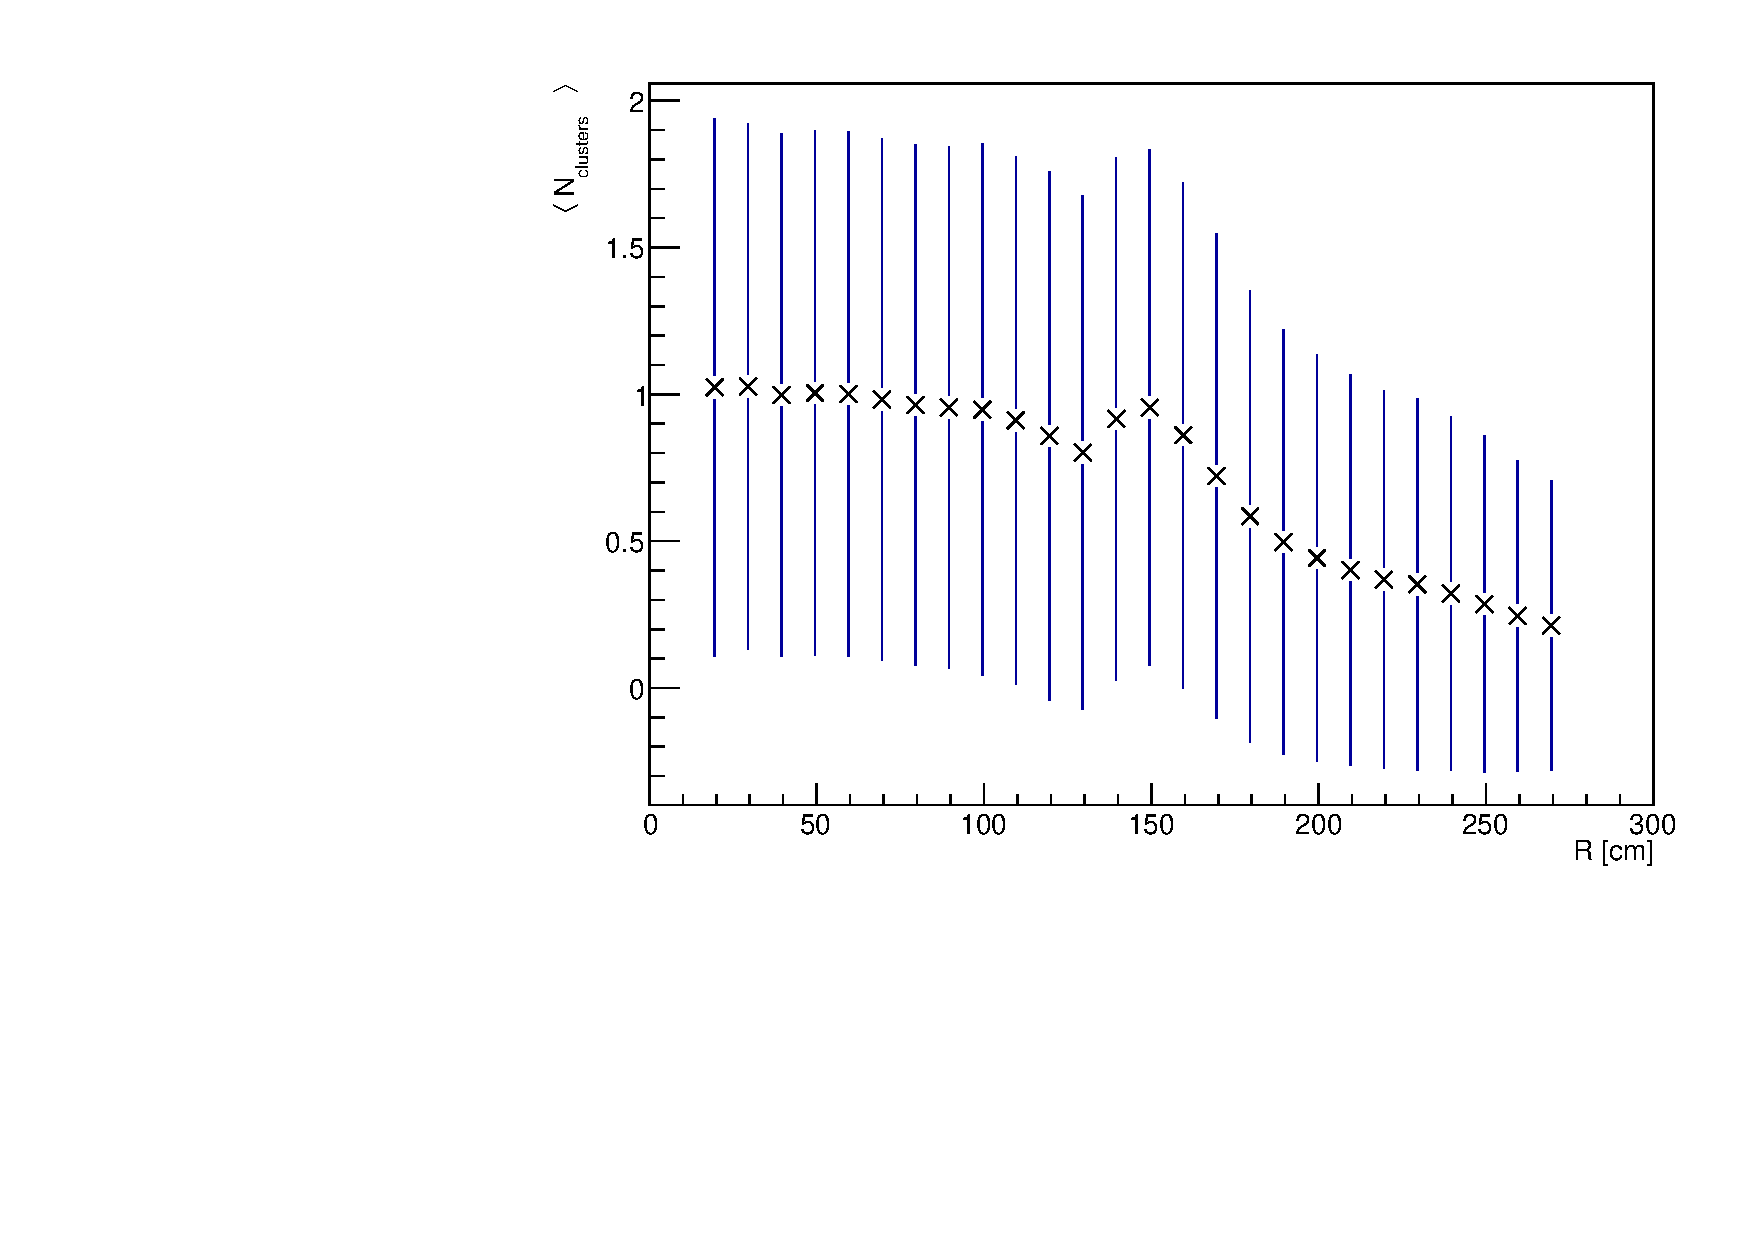
\includegraphics[width=.6\linewidth]{img/averageClusters.pdf}
    \caption{average clusters}
    \label{fig:work:average}
\end{figure}
labels too small
\begin{figure}[H]
    \centering
    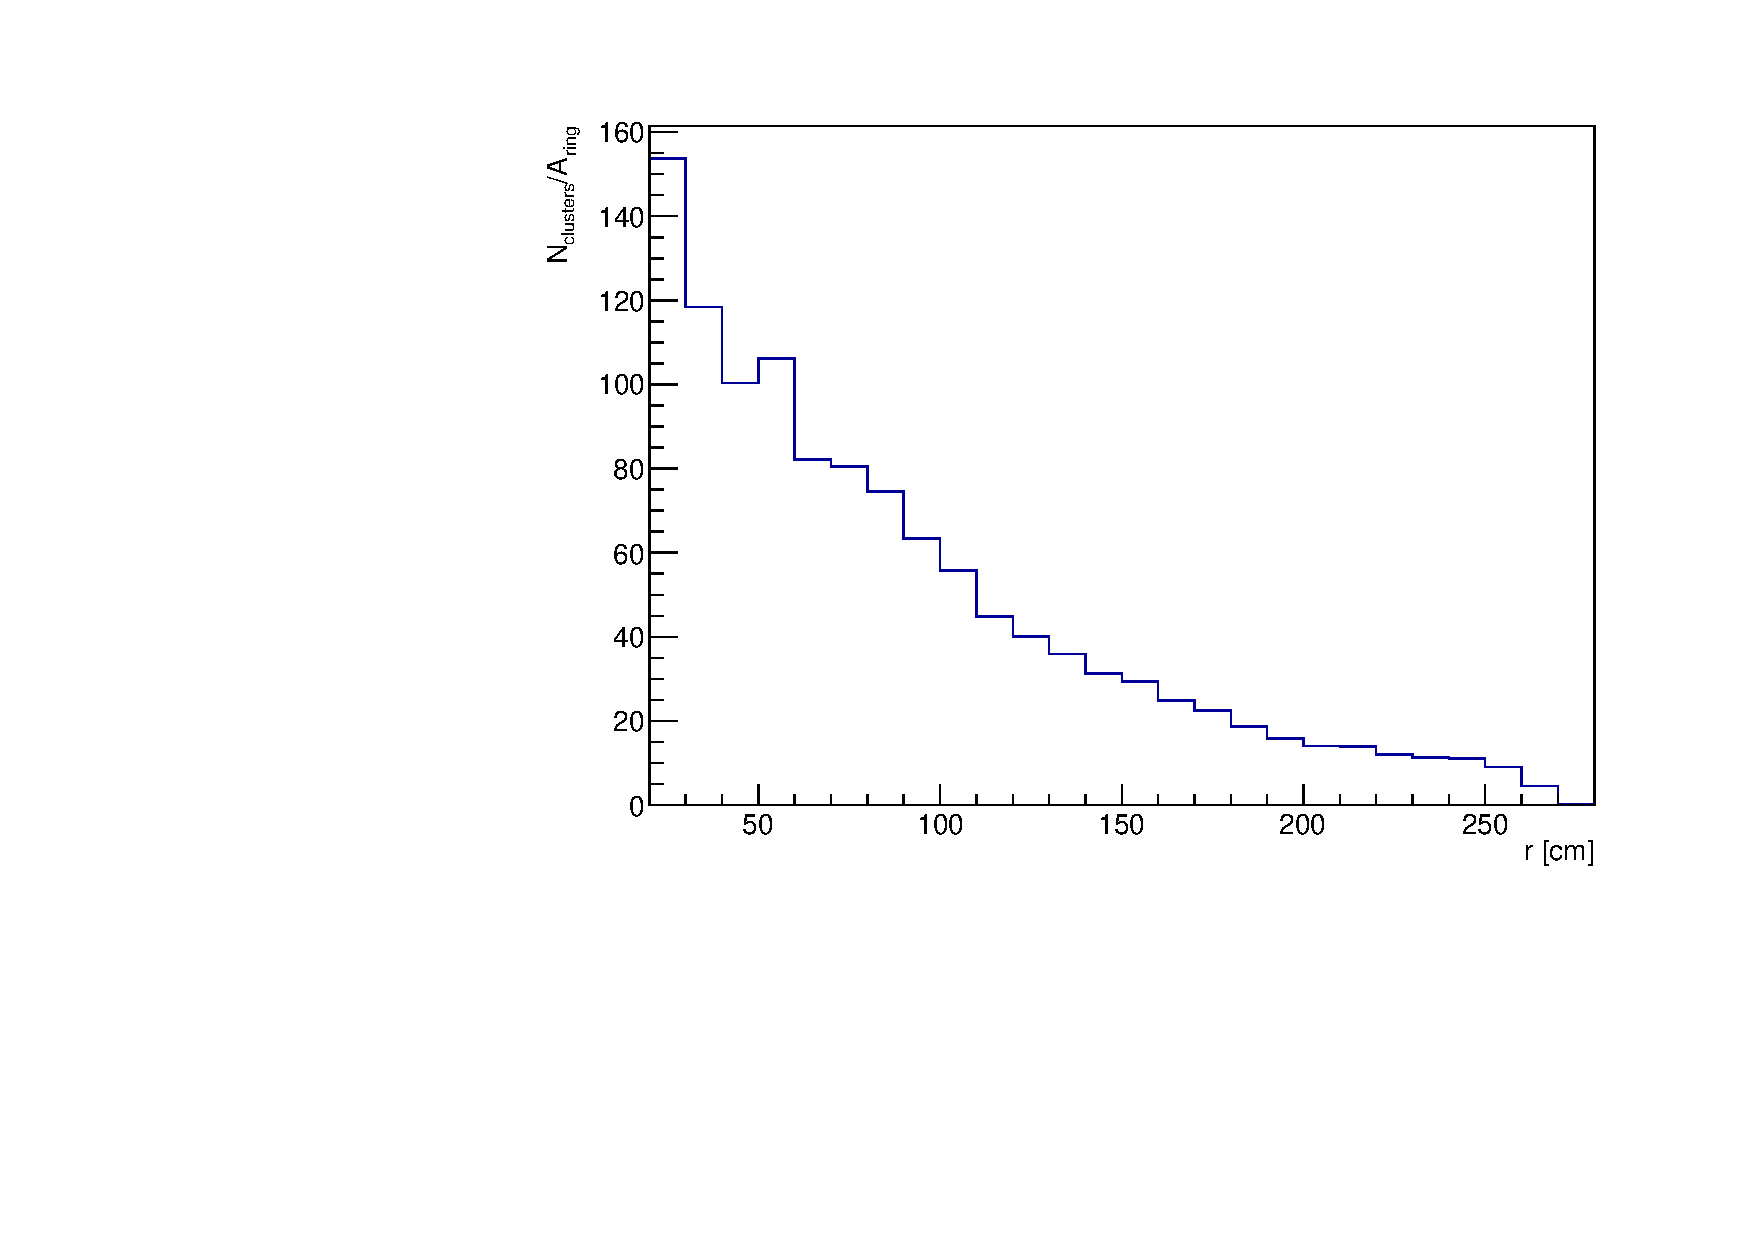
\includegraphics[width=.6\linewidth]{img/combined_clusters_norot.pdf}
    \caption{combined clusters}
    \label{fig:work:combined}
\end{figure}


\section{tilt?}
\begin{figure}[H]
    \begin{subfigure}{.48\linewidth}
        \centering
        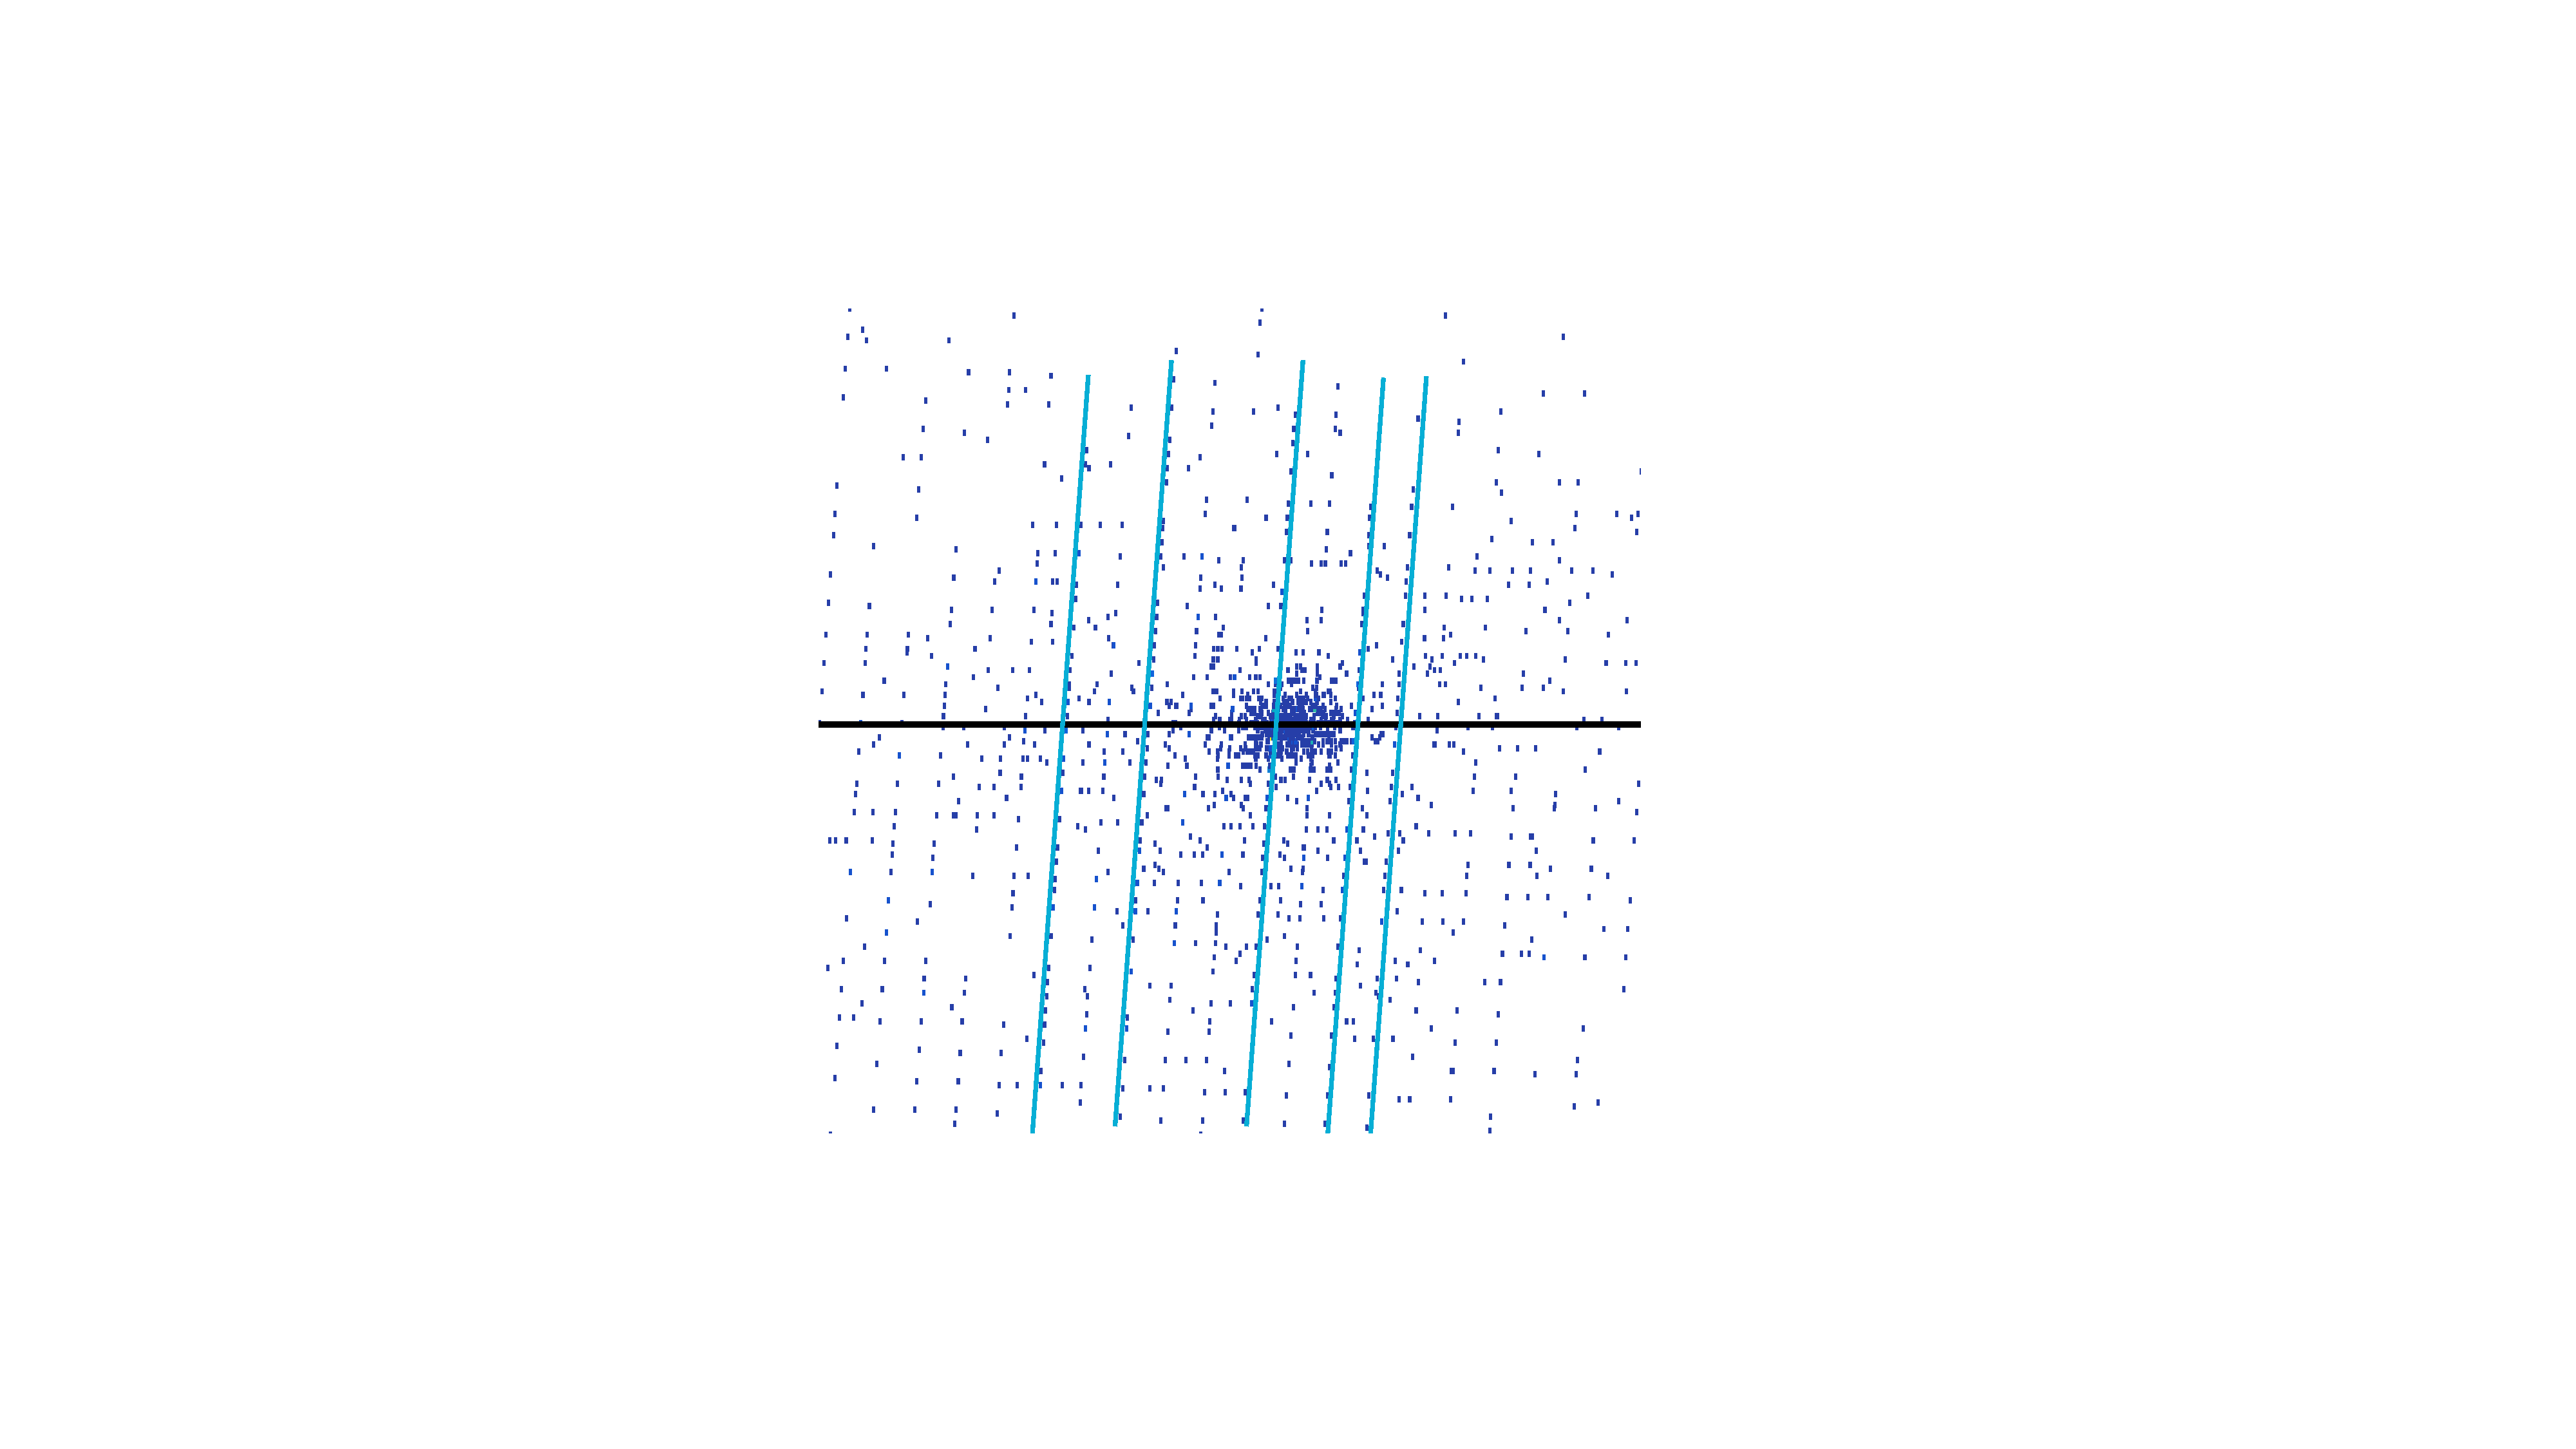
\includegraphics[width=\linewidth]{img/orig_config_clusters.pdf}
        \caption{before}
        \label{fig:work:tilt:before}
    \end{subfigure}
    \begin{subfigure}{.48\linewidth}
        \centering
        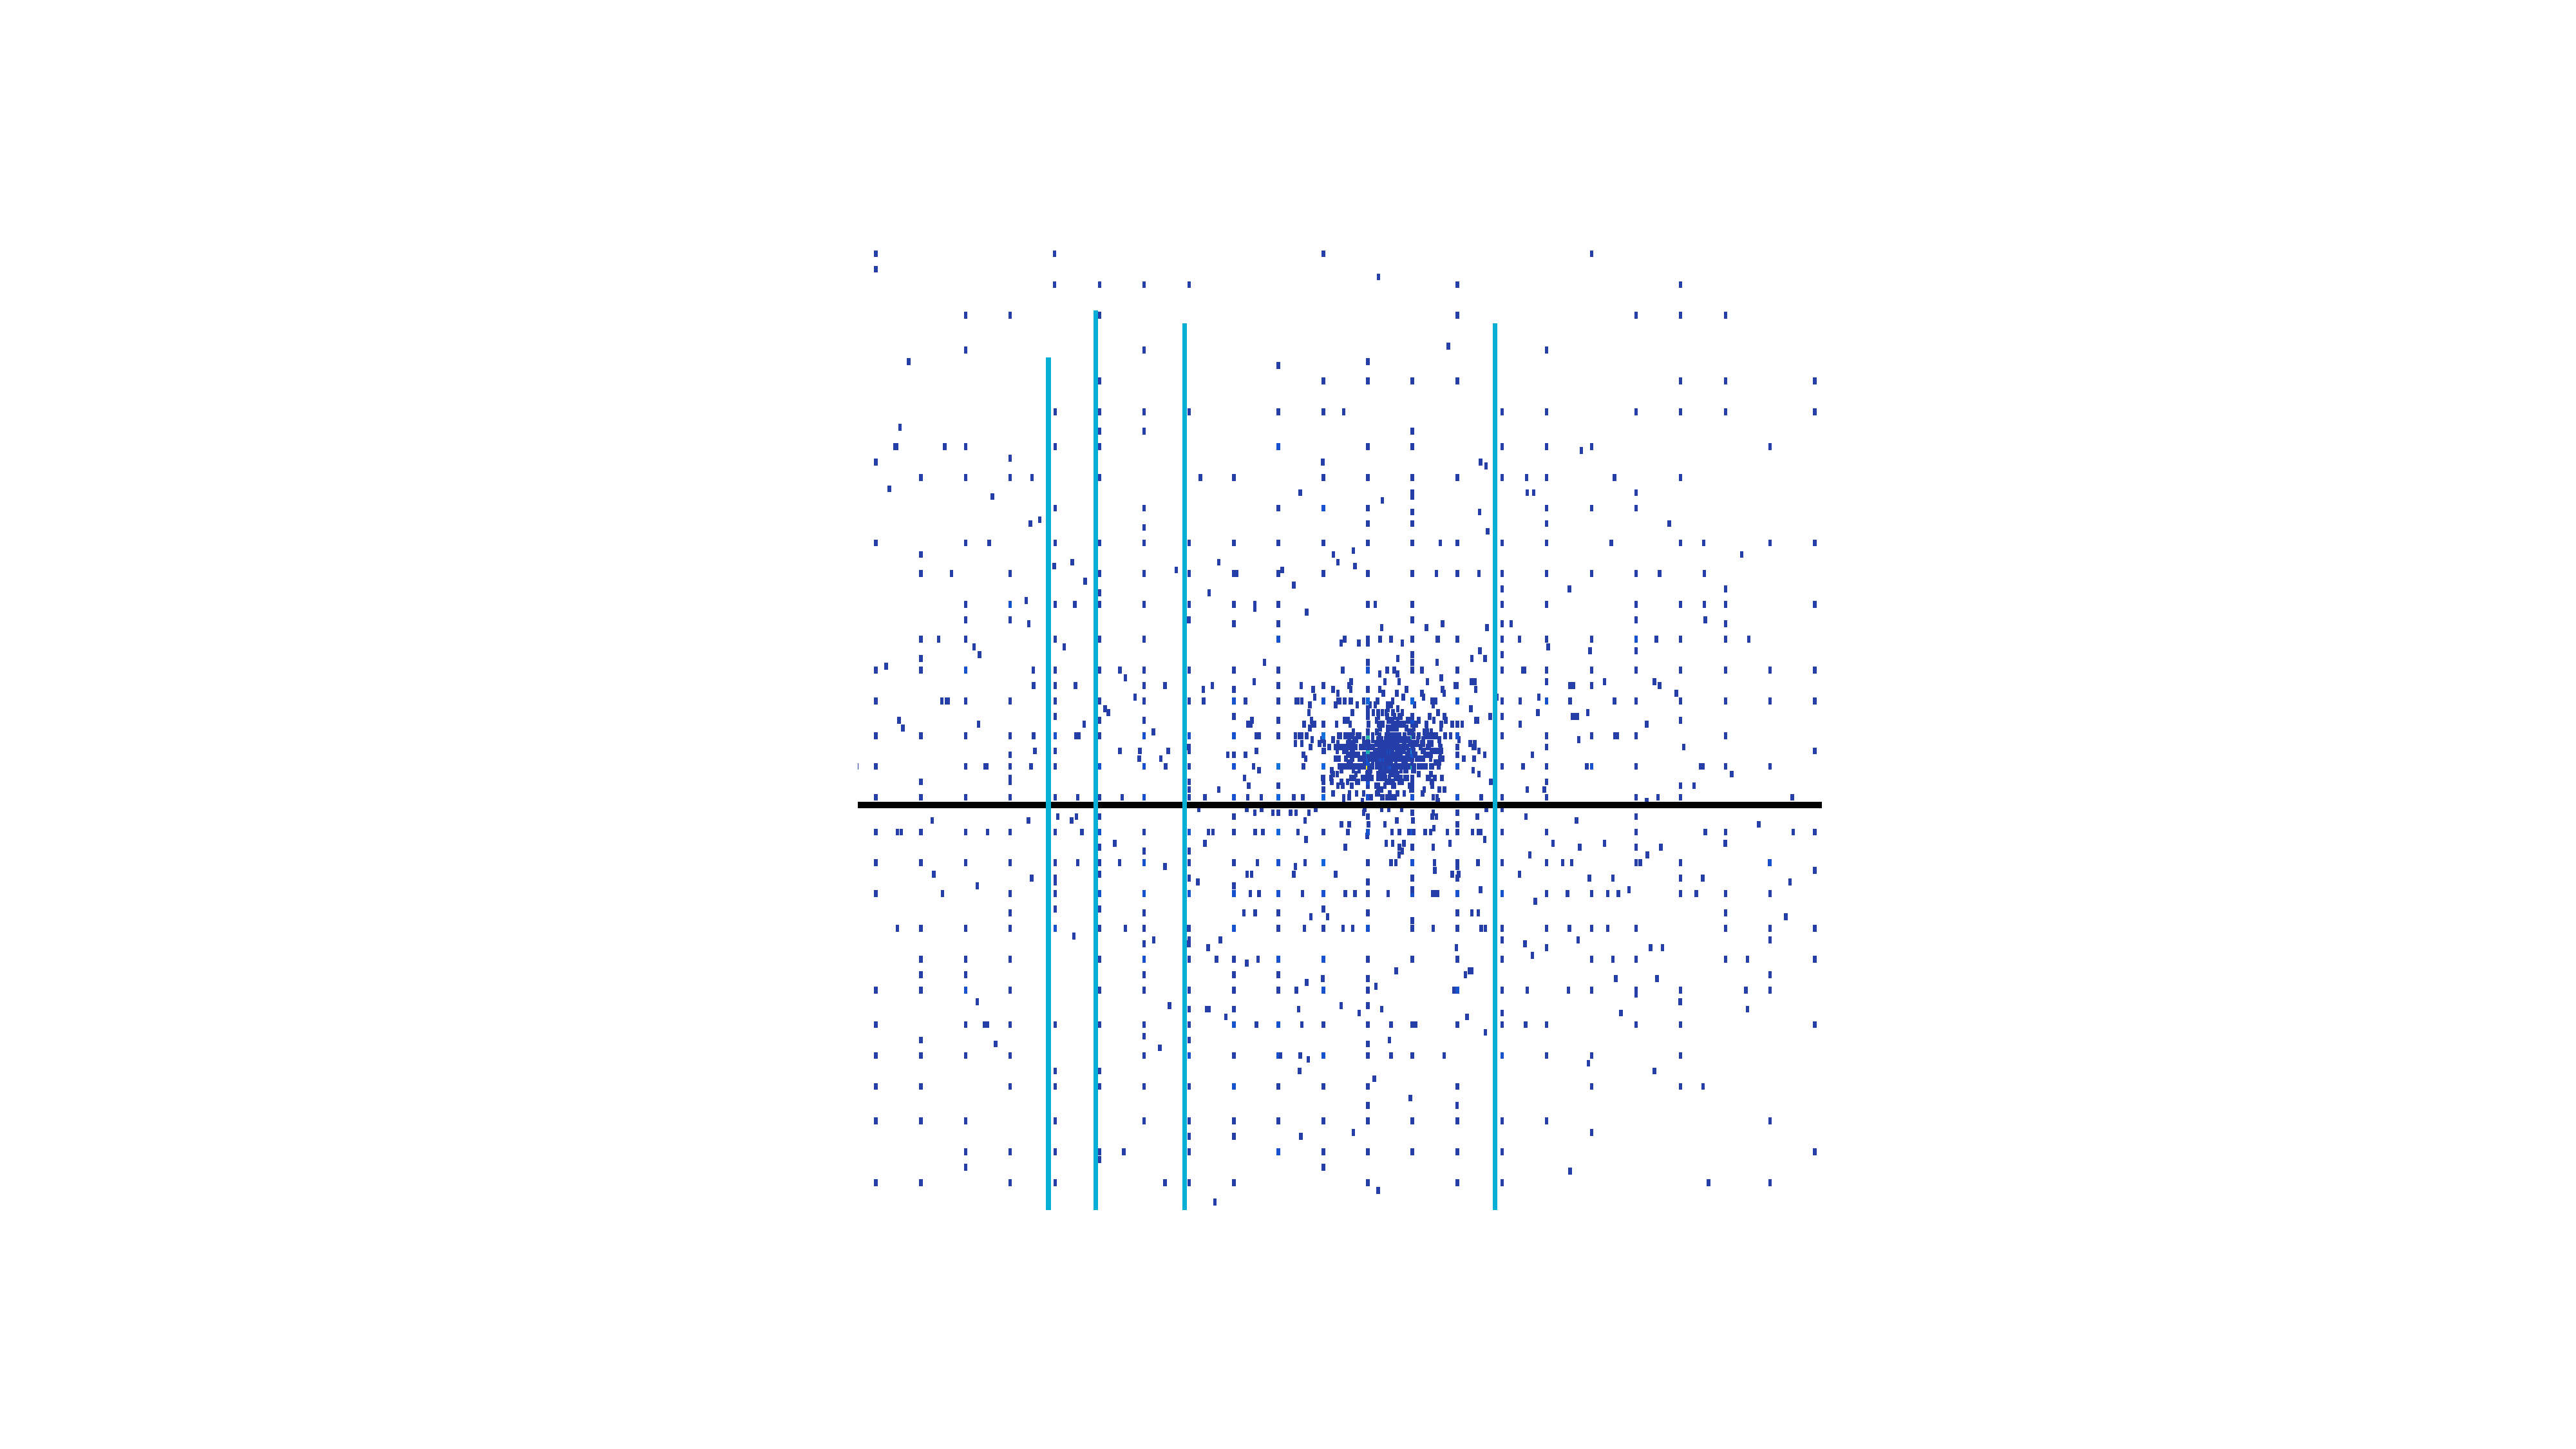
\includegraphics[width=\linewidth]{img/every_rot_removed_clusters.pdf}
        \caption{after}
        \label{fig:work:tilt:after}  
    \end{subfigure}
    \caption{need to level the lines, if decided to keep}
    \label{fig:work:tilt}
\end{figure}

\section{Sar$t$re MC generator}

\url{https://github.com/eic/SARTREdataset/blob/main/runcards/sartre_bnonsat_Au_phi.txt}

info about Campaign simulations

\section{phi - KK plots}